\chapter{Introduction}\label{chapter:introduction}
While the number of individuals that use blockchain systems is growing significantly, concerns about the performance and cost of using public blockchains like Ethereum \citep{buterin_2014} discourage widespread adoption. In particular, storing data in Ethereum is expensive. However, Decentralized Applications (DApps) running on top of the blockchain, usually manage some of their data on-chain. The narrow range of design patterns for fully Decentralized Applications \citep{wohrer_2021} and the lack of comprehensive research about on-chain data handling, hinders the development of efficient Smart Contracts (SCs) and leads to higher costs that are laid onto the users of DApps. Minimizing the use of SC storage in favor of more cost-efficient alternatives or using distributed file systems such as IPFS \citep{benet_2014} and Swarm \citep{tron_2020} alongside Ethereum, could ameliorate this problem.

According to this information, we define our research question: how can data be efficiently managed in Ethereum DApps?
In our attempt to answer this, we examine a wide range of storage options in Ethereum as well as a hybrid on-chain/off-chain architecture and make a comparative study to explore the advantages and disadvantages of each approach. 

{\bf Main contributions.} In this work, we:
\begin{itemize}[topsep=0pt, itemsep=0pt]
\item{Propose the use of the alternative data stores in Ethereum.}
\item{Cost-wise compare all available data stores.}
\item{Examine the time needed to retrieve data from the Ethereum blockchain.}
\item{Evaluate hybrid approaches utilizing IPFS and Swarm.}
\end{itemize}

Preliminary results of this research have been presented in~\citep{kostamis_2021}.
In the present work we broaden the analysis of the available on-chain data management methods and outline the impact that new Ethereum Improvement Proposals (EIPs) had on gas consumption. Specifically, we discuss the EIPs that were enforced after the Muir Glacier hard fork and introduced modifications related to the gas metering and refund mechanisms. Comments on the latter provide valuable insight on the cost of deleting data and serve to complement the discussion on data handling in SC storage.
Furthermore, we improve the evaluation of the retrieval performance 
of Ethereum by taking into account the fact that
recently retrieved data is cached by the operating system. Regarding the event-logs, additional remarks on the role that Bloom filters (BF) have in the data retrieval process, are made.
Finally, we enrich the discussion about the on-chain/off-chain
hybrid scheme with context about the cost of storing
the content identifiers in Ethereum.



The structure of this paper is as follows. In Section 2 we discuss the related work. In the next Section, we compare the available data handling practices for on-chain data and describe the main differences between IPFS and Swarm, from a theoretical point of view. In Section 4 we define the criteria of our experiments, outline the environment in which they were conducted and discuss our results both in terms of cost and performance. In the last Section, we gather our conclusions. 

\section{Background information on blockchain}\label{sec:}
\section{Background information on decentralized applications (dApps)}\label{sec:}
\section{Research question / motivation}\label{sec:}
\section{Thesis organization}\label{sec:organization}



% \indent write here


% \begin{figure}[h]
%     \begin{minipage}{0.5\textwidth}
%         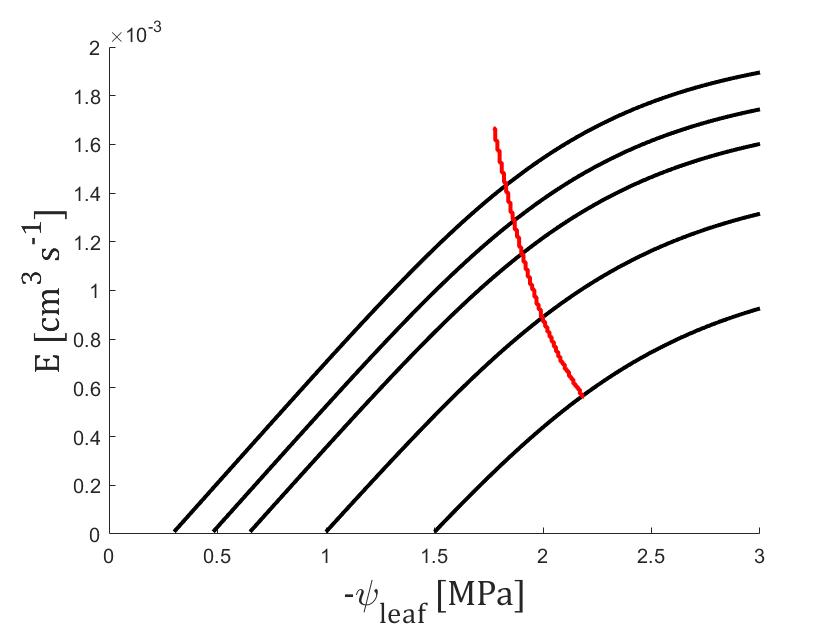
\includegraphics[width=0.9\linewidth, height=6cm]{./img/1_intro/random_figure.jpg}
%     \end{minipage}
%     \hfill
%     \begin{minipage}{0.5\textwidth}
%         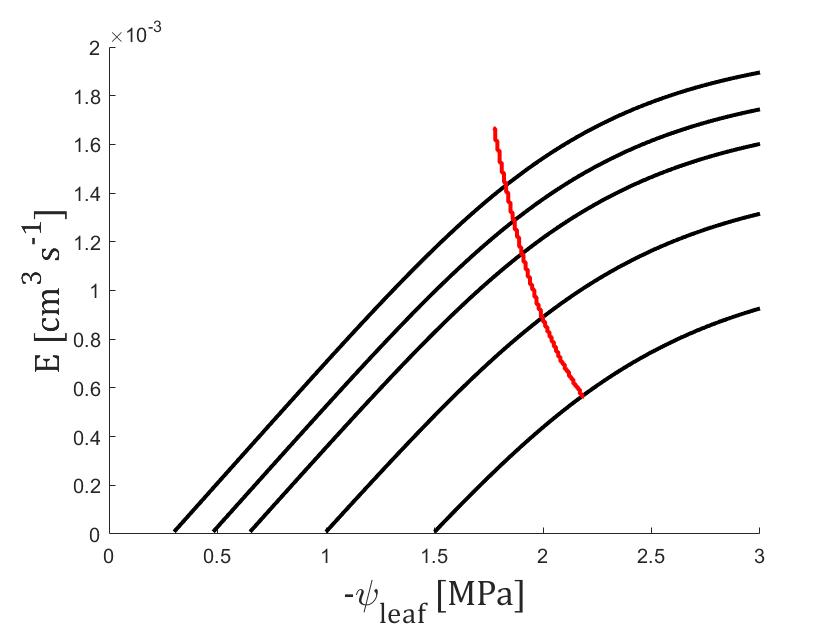
\includegraphics[width=1\linewidth, height=6cm]{./img/1_intro/random_figure.jpg}
%     \end{minipage}
%     \caption{If you want two figures next to each other}
%     \label{Figure:conceptually}
% \end{figure}

% or if you want just one 

% \begin{figure}[h]
%     \centering
%     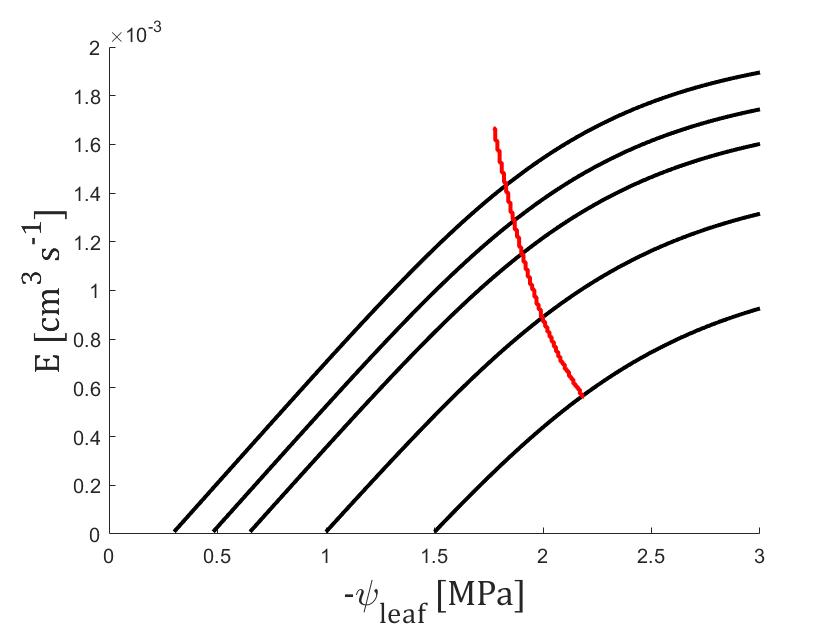
\includegraphics[width=0.5\linewidth, height=5cm]{./img/1_intro/random_figure.jpg}
%     \caption{If you want just one }
%     \label{Figure:just one }
% \end{figure}

% and you can reference it like this \ref{Figure:just one }

% \begin{table}[!h]
% \begin{center}
% \begin{tabular}{llcr} 
% \toprule
% & \textbf{parameter} & \textbf{type 1 } & \textbf{type 2 }\\
%  \midrule
%  \si{k_{0}}  & something & \SI{2e-05}{cm s^{-1}} &\SI{1e-03}{cm s^{-1}}\\
%   \si{h_{0}}  & other thing & \SI{-27.8}{cm} & \SI{-34.5}{cm}\\ 
%   \si{\tau} & exponent & 2 & 3 \\

% \bottomrule
% \end{tabular}
% \caption{This is how you make a table}
% \end{center}
% \end{table}
